%\documentclass[usenames,dvipsnames,notes]{beamer}
\documentclass[usenames,dvipsnames]{beamer}

\usetheme{uhh}
\showtotalframenumber
\showuhhlogoeachframe
\showsections

\usepackage{ textcomp }
\usepackage{booktabs}
\usepackage{xcolor}
\usepackage{amsmath}
\usepackage{graphicx}
\usepackage{tabularx}
\usepackage{color}
\DeclareMathOperator*{\argmin}{arg\,min}

\usepackage{listings}
\lstset{
  language=python
  }



\DeclareMathOperator{\tf}{tf}
\DeclareMathOperator{\tfidf}{tf-idf}
\DeclareMathOperator{\coverage}{coverage}
\DeclareMathOperator{\dist}{dist}
\DeclareMathOperator{\SPD}{SPD}
\DeclareMathOperator{\pscore}{\mathit{p}-score}
\DeclareMathOperator{\gold}{gold}
\DeclareMathOperator{\LCH}{LCH}
\DeclareMathOperator{\hscore}{\mathit{h}-score}
\DeclareMathOperator{\hpcscore}{\mathit{hpc}-score}
\DeclareMathOperator{\hpcavg}{\mathit{hpc}-avg}
\DeclareMathOperator{\cbadnessval}{\mathit{c}-badness}
\DeclareMathOperator{\hbadnessval}{\mathit{h}-badness}
\DeclareMathOperator{\badnessval}{badness}
\DeclareMathOperator{\pvalue}{\mathit{p}-value}



\title{Improving Hypernymy Extraction with Distributional Semantic Classes}

\author[Panchenko et al. LREC'18]{\underline{Alexander Panchenko}, Dmitry Ustalov, Stefano Faralli, Simone Paolo Ponzetto, and Chris Biemann}
% \institute{$^1$ University of Hamburg, Department of Informatics, Language Technology Group, Germany \\
%         $^2$ University of Mannheim, School of Business Informatics and Mathematics, Data and Web Science Group} 
\date[10.05.2018]{May 10, 2018}

\AtBeginSection[]
{
   %%%%% section title
   % This is how it would look like in Beamer:
   % \begin{frame}
   %     \frametitle{Overview}
   %     \tableofcontents[sections={2-3},currentsection,sectionstyle=show/hide,subsectionstyle=hide]
   % \end{frame}
  \begin{frame}[plain]
  \begin{tikzpicture}[overlay]
    \relax%
    \fill[blueuhh,opacity=1] (-10,-10)
    rectangle(\the\paperwidth,\the\paperheight);
  \end{tikzpicture}
   \begin{tikzpicture}[overlay]
    \relax%
    \fill[white,opacity=1] (-5,-1.2)
    rectangle(\the\paperwidth,0.5) node[pos=0.5,black]{\LARGE\insertsectionhead};
  \end{tikzpicture}
  \end{frame}

  %%%% add subsection to show navigation dots
  \subsection{}
}


\begin{document}

\maketitle

%
\section{Overview}

\begin{frame}
  \frametitle{Overview}

  \begin{itemize}
		\item \alert{\textbf{Inducing word sense representations}}:
		\begin{itemize}
		\item \textbf{word sense embeddings via retrofitting} \cite{pelevina-EtAl:2016:RepL4NLP,remus:2018};
		\item \textbf{inducing synsets}~\cite{ustalov-panchenko-biemann:2017:Long,ustalov2017fighting,madoc43362}
		\item \textbf{inducing semantic classes} \cite{panchenko:2018:SemanticClasses} 
		\end{itemize}
	
	
	
	\pause 
	\vspace{1em}
	\item \alert{\textbf{Making induced senses interpretable}} \cite{panchenko-EtAl:2017:EMNLP2017Demos,panchenko-EtAl:2017:EACLlong}
	
	\pause
	\vspace{1em}
	\item \alert{\textbf{Linking induced word senses to lexical resources}}~\cite{panchenko2016best,faralli2016linked,panchenko-EtAl:2017:SENSE2017,biemann2018framework}	
			
\end{itemize}
	
\end{frame}

\section{Introduction}
\subsection{}


\begin{frame}{Hypernyms}

\begin{block}{Examples of hypernymy relations}
\begin{itemize}
	\item \textbf{apple} --isa\textrightarrow \textbf{ fruit}
	\item \textbf{mangosteen} --isa\textrightarrow \textbf{ fruit}
\end{itemize}
\end{block}

\pause

\begin{block}{Examples of applications of hypernyms}
\begin{itemize}
	\item question answering~\cite{Zhou:13} 
	\item query expansion~\cite{gong2005web}
	\item semantic role labelling~\cite{shi2005putting} 
\end{itemize}
\end{block}
\end{frame}

%Hypernyms are useful in various applications, such as .
% Hypernyms are also the building blocks for learning taxonomies from text~\cite{bordea2016semeval}. Consider the following sentence: ``This caf\'e serves fresh \textit{mangosteen} juice''. Here the infrequent word ``mangosteen'' may be poorly represented or even absent in the vocabulary of a statistical model, yet it can be substituted by lexical items with better representations, which carry close meaning, such as its hypernym ``fruit'' or one of its close co-hyponyms, e.g. ``mango''. 

\begin{frame}{Automatic extraction of hypernyms}

% Currently available approaches to hypernymy extraction focus on the acquisition of individual binary hypernymy relations~\cite{hearst1992automatic,snow2004learning,weeds2014learning,shwartz-goldberg-dagan:2016:P16-1,glavavs-ponzetto:2017:EMNLP2017}. Frequencies of the extracted relations usually follow a power-law, with a long tail of noisy extractions containing rare words. We propose a method that performs post-processing of such noisy binary hypernyms using distributional semantics, cf. Figure~\ref{fig:cosetbinary}. Namely, we use the observation that distributionally related words are often are co-hyponyms~\cite{wandmacher2005semantic,Heylen:08} and operationalize it to perform filtering of noisy relations by finding dense graphs composed of both hypernyms and co-hyponyms.  
 
% The contribution of the paper is an unsupervised method for post-processing of noisy hypernymy relations based on  clustering of graphs of word senses induced from text. The idea to use distributional semantics to find hypernyms seems natural and has been widely used. However, the existing methods used distributional, yet \textit{sense-unaware} and \textit{local} features. We are the first to use \textit{global sense-aware distributional structure} via the induced semantic classes to improve hypernymy extraction. The implementation of our method and the induced language resources (distributional semantic classes and cleansed hypernymy relations) are available online.\footnote{\url{https://github.com/uhh-lt/mangosteen}}


%In her pioneering work, \newcite{hearst1992automatic} proposed to extract hypernyms based on lexical-syntactic patterns from text. \newcite{snow2004learning} learned such patterns automatically based on a set of hyponym-hypernym pairs. \newcite{pantel2006espresso} presented another approach for weakly supervised extraction of similar extraction patterns. These approaches use some training pairs of hypernyms to bootstrap the pattern discovery process. For instance, \newcite{sang2007extracting} used web snippets as a corpus for extraction of hypernyms. More recent approaches exploring the use of distributional word representations for extraction of hypernyms and co-hyponyms include~\cite{roller2014inclusive,weeds2014learning,necsulescu2015reading,vylomova-EtAl:2016:P16-1}. They rely on two distributional vectors to characterize a relation between two words, e.g. on the basis of the difference of such vectors or their concatenation. \newcite{Levy:15} discovered a tendency to lexical memorization of such approaches, hampering their generalization to other domains.
%
%\newcite{fu2014learning} relied on an alternative approach where a projection matrix is learned, which transforms a distributional vector of a hyponym to the vector of its hypernym. \newcite{ustalov-EtAl:2017:EACLshort} improved this method by adding regularizers in the model that take into account negative training samples and the asymmetric nature of the hypernyms. 
%
%Recent approaches to hypernym extraction focused on learning \textit{supervised} models based on a combination of syntactic patterns and distributional features~\cite{shwartz-goldberg-dagan:2016:P16-1}. Note that while methods, such as \cite{mirkin-dagan-geffet:2006:POS} and \cite{shwartz-goldberg-dagan:2016:P16-1} use distributional features for extraction of hypernyms, in contrast to our method, they do not take into account word senses and    global distributional structure. 
%
%\newcite{seitner2016large} performed extraction of hypernyms from the web-scale Common Crawl\footnote{\url{http://www.commoncrawl.org}} text corpus to ensure high lexical coverage. In our experiments, we use this web-scale database of noisy hypernyms, as the large-scale repository of automatically extracted hypernyms to date. 

\end{frame}


\begin{frame}{Induction of semantic classes}

%This line of research starts with \cite{Lin2001}, where sets of similar words are clustered into concepts. While this approach performs a hard clustering and does not label clusters, these drawbacks are addressed in \cite{Pantel2002}, where words can belong to several clusters, thus representing senses, and in \cite{Pantel2004}, where authors aggregate hypernyms per cluster, which come from Hearst patterns. The main difference to our approach is that we explicitly represent senses both in clusters and in their hypernym labels, which enables us to connect our sense clusters into a global taxonomic structure. Consequently, we are the first to use semantic classes to improve hypernymy extraction. 
%
%\newcite{ustalov-panchenko-biemann:2017:Long} proposed a synset induction approach based on global clustering of word senses. The authors used the graph constructed of dictionary synonyms, while we use distributionally-induced graphs of senses.

\end{frame}


\begin{frame}{Main contributions}

\begin{itemize}
	\item We show how distributionally-induced \alert{\textbf{semantic classes}} can be helpful  for \alert{\textbf{extracting hypernyms}}:
	\pause
	\vspace{10pt}
	\begin{enumerate}
		\item A method for \alert{inducing sense-aware semantic classes} using distributional semantics; 
		\vspace{10pt}
		\item A method for using the induced semantic classes for \alert{filtering noisy hypernymy relations}.
	 \end{enumerate}
\end{itemize}
\end{frame}

\section{Method}
\subsection{}


\begin{frame}{ Labeled semantic classes}

\begin{figure}[ht]
  \centering
  \includegraphics[width=.99\textwidth]{figures/coset}

\end{figure}

\begin{itemize}
\item \alert{Post-processing of hypernymy relations} using distributionally induced semantic classes;
\item A semantic class is a clusters of induced word senses \alert{labeled with hypernyms}.

\end{itemize}

\note{The word postfix, such as \texttt{\#1}, is an ID of an induced sense. The wrong hypernyms outside the cluster labels are removed, while the missing ones not present in the noisy database of hypernyms are added. }


\end{frame}


\begin{frame}{Outline of our approach}



\begin{enumerate}
	\item Sense-aware distributional semantic classes are \textbf{induced from a text corpus}; 
	\item Semantic classes are used to \textbf{filter a noisy hypernyms} database. 
 
\end{enumerate}

\pause 


\begin{figure}
  \centering
  \includegraphics[width=.99\textwidth]{figures/outline}
  \end{figure}


\note{(e.g. extracted by an external method from a text corpus)}

\end{frame}


\begin{frame}{Chinese Whispers graph clustering}

Used for word sense induction, used for global clustering ... 

\end{frame}

	
\begin{frame}{Sample of induced sense inventory}


\begin{table}
\centering
\scriptsize
\begin{tabular}{l|p{6cm}|p{2.5cm}} 
\bf Word Sense & \bf Local Sense Cluster: Related Senses & \bf Hypernyms \\
\toprule
 mango\#0 &  peach\#1, grape\#0, plum\#0, apple\#0, apricot\#0, watermelon\#1, banana\#1, coconut\#0, pear\#0, fig\#0, melon\#0,  \textbf{mangosteen\#0}, ... & fruit\#0, food\#0, ... \\
 
\midrule
apple\#0 & mango\#0, pineapple\#0, banana\#1, melon\#0, grape\#0, peach\#1, watermelon\#1, apricot\#0, cranberry\#0, pumpkin\#0, \textbf{mangosteen\#0}, ... & fruit\#0, crop\#0,  ... \\

\midrule
Java\#1 & C\#4, Python\#3, Apache\#3, Ruby\#6, Flash\#1, C++\#0, SQL\#0, ASP\#2, Visual Basic\#1, CSS\#0, Delphi\#2, MySQL\#0, Excel\#0, Pascal\#0, ... & programming language\#3, language\#0, ... \\

\midrule
Python\#3 & PHP\#0, Pascal\#0, Java\#1, SQL\#0, Visual Basic\#1, C++\#0, JavaScript\#0, Apache\#3, Haskell\#5, .NET\#1, C\#4, SQL Server\#0, ... & language\#0, technology\#0, ... \\

\end{tabular}


\end{table}


\note{ entries  representing ``fruits'' and ``programming language'' senses. Each word sense $s$ is represented with a list of related senses $\mathcal{N}(s)$ and the list of hypernyms $\mathcal{H}(s)$. The hypernyms can be used as human-interpretable sense labels of the sense clusters. One sense $s$, such as ``apple\#0'', can appear in multiple entries.}

\end{frame}


\begin{frame}{Sample of induced  semantic classes}


\begin{table}
\centering
\scriptsize
\begin{tabular}{l|p{2.5in}|p{1in}} 
\bf ID &  \bf Global Sense Cluster: Semantic Class & \bf Hypernyms \\ 

\toprule

1 & peach\#1, banana\#1, pineapple\#0, berry\#0, blackberry\#0, grapefruit\#0, strawberry\#0, blueberry\#0, \alert{mango\#0}, grape\#0, melon\#0, orange\#0, pear\#0, plum\#0, raspberry\#0, watermelon\#0, \alert{apple\#0}, apricot\#0, watermelon\#0, pumpkin\#0, berry\#0, \alert{\textbf{mangosteen\#0}}, ...  & vegetable\#0, fruit\#0, crop\#0, ingredient\#0, food\#0, $\cdot$ \\ 

\midrule

2  & C\#4, Basic\#2, Haskell\#5, Flash\#1, \alert{Java\#1}, Pascal\#0, Ruby\#6, PHP\#0, Ada\#1, Oracle\#3, \alert{Python\#3}, Apache\#3, Visual Basic\#1, ASP\#2, Delphi\#2, SQL Server\#0, CSS\#0, AJAX\#0, JavaScript\#0, SQL Server\#0, Apache\#3, Delphi\#2, Haskell\#5, .NET\#1, CSS\#0, ... & programming language\#3, technology\#0, language\#0, format\#2, app\#0
\end{tabular}

\note{Sample of the induced  sense clusters representing ``fruits'' and ``programming language'' semantic classes. Similarly to the induced word senses, the semantic classes are labeled with hypernyms. In contrast to the induced word senses, which represent a local clustering of word senses (related to a given word) semantic classes represent a global sense clustering of word senses. One sense $c$, such as ``apple\#0'', can appear only in a single cluster.}


\end{table}

\end{frame}

%\begin{frame}{A non-coherent ego network}
%
%\begin{figure}
%  \centering
%  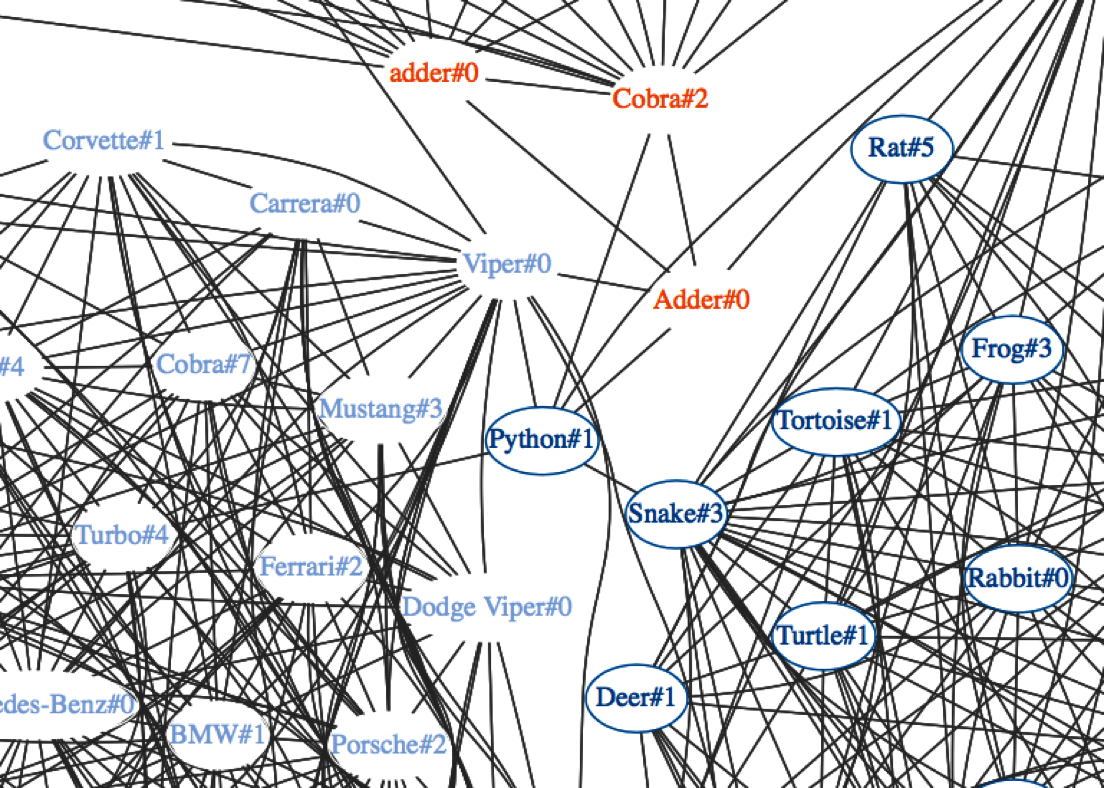
\includegraphics[width=.99\textwidth]{figures/ego-network}
%\end{figure}
%
%\note{An example of a non-coherent ego network  of the automatically induced sense \texttt{Python\#1}, representing the ``animal" sense. We prune it to remove terms not relevant to the animal sense. }
%  	
%\end{frame}

\begin{frame}{Network of induced word senses}
	
	
\begin{figure}[ht]
  \centering
  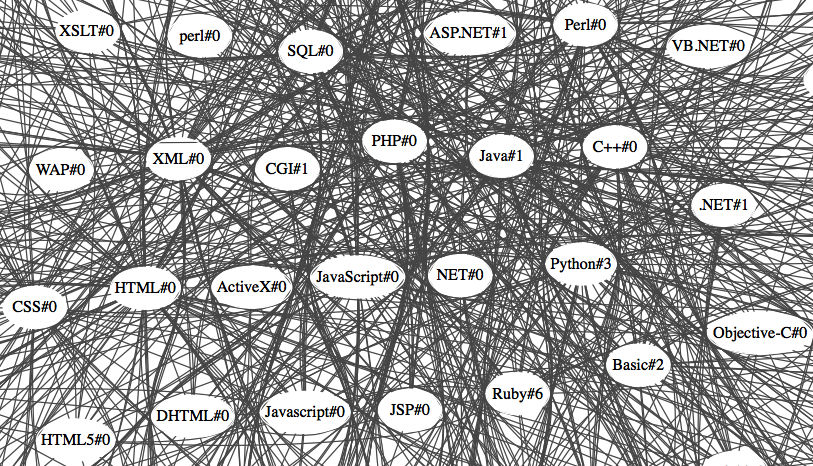
\includegraphics[width=.99\textwidth]{figures/cluster-programming}
\end{figure}

  \note{Senses referring to programming languages co-occur in global sense cluster entries, resulting in a densely connected set of co-hyponyms. }

\end{frame}

% extra slide ...

\section{Optimization of meta-parameters}
\subsection{}
\begin{frame}{Comparison to WordNet and BabelNet}

\begin{block}{Meta-parameters}	
\begin{enumerate}
\item \textbf{Min. sense co-occurrences}: $t > 0$
\item \textbf{Sense edge weight}: count or log(count) 
\item \textbf{Hypernym weight type}: tf-idf or tf
\end{enumerate}
\end{block}

\pause 

% & $\hpcavg$, \textbf{WordNet} & $\hpcavg$, \textbf{BabelNet

$$
  \hpcscore(c) = \frac{\hscore(c) + 1}{\pscore(c) + 1} \cdot \coverage(c)\text{.}
$$

$$
  \pscore(c) = \frac{1}{\left\vert{}c\right\vert} \sum^{\left\vert{}c\right\vert}_{i=1} \sum^i_{j=1} \dist(w_i, w_j)\text{.}
  \hscore(c) = \frac{\left\vert\mathcal{H}(c) \cap \gold(c)\right\vert}{\left\vert\mathcal{H}(c)\right\vert}\text{.}
$$
	
\note{
The method has really just a few parameters, but still we wanted to know their impact... 

Since we are in an unsupervised setting...

Performance of different configurations of the hypernymy labeled global sense clusters in terms of their similarity to WordNet/BabelNet. The results are sorted by performance on BabelNet dataset, the best values in each section are boldfaced. The two underlined configurations are respectively the best \textit{coarse-grained} and \textit{fine-grained} grained semantic class models used in all experiments. The coarse grained model contains less semantic classes, but they tend to be more consistent than those of the fine-grained model, which contains more senses and classes. }

	
\end{frame}


\begin{frame}{Best coarse- and fine-grained models}


\begin{table}
\scriptsize
\centering
\begin{tabular}{p{1.4cm}|p{1.2cm}|p{1.2cm}|p{1.3cm}|p{1.1cm}|p{1.2cm}|p{1.2cm}}
  \textbf{Min. sense co-occurr.}, $t$ & \textbf{Edge weight}, $E$ & \textbf{Hypernym weight}, $H$ & \textbf{Number of clusters} & \textbf{Number of senses} & $\hpcavg$, \textbf{WordNet} & $\hpcavg$, \textbf{BabelNet} \\ \toprule

100 & log  & tf-idf & 734  &  18\,028 & 0.092 & 0.304 \\

0  & count  & tf-idf & 1870 & 208\,871 & 0.041 & 0.279 \\
 
\end{tabular}

\end{table}

	
\end{frame}


\section{Results}
\subsection{}

\begin{frame}{ ... }

\end{frame}


\begin{frame}{ ... }

\end{frame}


\begin{frame}{ ... }

\end{frame}


\begin{frame}{ ... }

\end{frame}


\begin{frame}{ ... }

\end{frame}



\begin{frame}{ ... }

\end{frame}


\begin{frame}{ ... }

\end{frame}


\begin{frame}{ ... }

\end{frame}


\begin{frame}{ ... }

\end{frame}


\bibliography{biblio}
\bibliographystyle{apalike2}


\end{document}

